\RequirePackage{plautopatch}
\documentclass[a4j,dvipdfmx,
%,draft%
]{jsbook}
\setlength{\textwidth}{\fullwidth}
\setlength{\evensidemargin}{\oddsidemargin}

%% 表題の設定
\makeatletter
% 1ページ用
\newcommand\ktitle{数値解析ノート}
% 途中で表示するとき用(1行)
\newcommand\ktitles{\ktitle}
\makeatother

% !TEX root = main.tex
%

% チェック
\RequirePackage[l2tabu, orthodox]{nag}

%% パッケージ
%図
\usepackage[hiresbb]{graphicx}
\usepackage{caption}
\usepackage[subrefformat=parens]{subcaption}
%数式
\usepackage{amsmath}
\usepackage[all, warning]{onlyamsmath}
\allowdisplaybreaks
\def\equation{\gather}%%hyperref対応
\def\endequation{\endgather}%%hyperref対応
\usepackage{amssymb}
\usepackage{amsthm}
\newcommand{\hmmax}{0}
\newcommand{\bmmax}{0}
\usepackage{bm}
%SI単位系
\usepackage{siunitx}
%表
\usepackage{longtable}
%アルゴリズム
\usepackage[chapter]{algorithm}
\usepackage{algorithmicx}
\usepackage{algpseudocode}
%ソースコード
\usepackage{listings,extern/plistings/plistings}
\lstset{
    numbers=left,
    numberstyle=\footnotesize,
    basicstyle=\footnotesize,
    breaklines=true,
    frame={tb},
    flexiblecolumns=true
}
%URL
\usepackage{url}
\urlstyle{rm}
%しおり
\usepackage{bookmark}
%引用
\usepackage{cite}%下の3行がない限りhyperrefとは同時に使わない.
\makeatletter
\def\NAT@parse{\typeout{This is a fake Natbib command to fool Hyperref.}}
\makeatother
%ハイパーリンク
\usepackage{hyperref}%なるべく後
\usepackage{pxjahyper}%日本語対応
\renewcommand\UrlFont{\rmfamily}
%フォント(※順番を変えない.)
\usepackage[nomath]{lmodern}
\usepackage[T1]{fontenc}
\usepackage{textcomp}
\usepackage{newtxmath}
%自分のパッケージ(他のパッケージに依存するから最後にする)
\usepackage[book,amsthm,many]{kmath}
\usepackage{kmacro}

%タイトル
\title{\ktitle}
\author{椛島 健太}
\西暦
%hypersetup用の設定
\hypersetup{%
    bookmarksnumbered=true,%
    setpagesize=false,%
    pdftitle={\ktitles},%
    pdfauthor={椛島 健太},%
    pdfsubject={},%
    pdfkeywords={},%
    hidelinks,%
    pdfstartview=FitH,%
    pdfremotestartview=FitH%
}

%参考文献
\def\bibname{参考文献}

%数式の番号(章番号を使うようにする.)
\makeatletter
\renewcommand{\theequation}{%
\arabic{chapter}.\arabic{equation}%
}
\@removefromreset{equation}{section}
\@addtoreset{equation}{chapter}
\makeatother
 % 設定を読みこむ

\begin{document}

% タイトルページ
\maketitle

% copyright ページ
\thispagestyle{empty}
\null\vfill % 文章をページの下に寄せる
\noindent
\copyright \ 2021, Kenta Kabashima.\\
This work is licensed under the Creative Commons Attribution-ShareAlike 4.0 International License. To view a copy of this license, visit
\url{http://creativecommons.org/licenses/by-sa/4.0/}.

% 目次ページ
\setcounter{tocdepth}{2}
\tableofcontents

% !TEX root = main.tex
%

\chapter{本書について}

本書では,私が数値解析関係で調査したことをまとめる.
基本的には,実装のためにアルゴリズムやその理論を確認した結果をまとめることを目的としており,
C++ で実装したものは Git リポジトリ \cite{NumericalCollectionCpp} にて公開している.

数値解析の分野も幅広く,
扱う対象によって独特の記号が定義されるケースが少なくない,
そこで,本書では部または章ごとに記号の定義を記載している.

% !TEX root = ../main.tex
%

\part{求根アルゴリズム}

\chapter{導入}

求根アルゴリズム (root-finding algorithm)
は,微分などの演算を含まない通常の方程式
$f(\bm{x})=\bm{0}$ ($f : \setR^n \to \setR^m$)
の解を求めるためのアルゴリズムである.
関数 $f$ の種類に依り様々な手法が存在する.

\chapter{記号}

本部で使用する記号を以下に示す.

\begin{explainlist}
    $\setR$ & 実数の集合 \\
    $f'(x)$ & 1 変数関数 $f : \setR \to \setR$ の微分係数 \\
    $\nabla f$ & 関数 $f : \setR^n \to \setR$ の勾配 \\
    $\frac{\partial \bm{f}}{\partial \bm{x}}$ & 関数 $\bm{f} : \setR^n \to \setR^n$ の Jacobian \\
    $\|\bm{x}\|_2$ & ベクトル $\bm{x}$ の 2-ノルム \\
\end{explainlist}

% !TEX root = ../main.tex
%

\chapter{Newton-Raphson 法}\label{chap:root-finding_newton-raphson}

Newton-Raphson 法は,
次の式のような更新式で反復的に方程式 $f(x) = 0$ の根を求める手法である.
\begin{equation}
    x_{n+1} = x_n - \frac{f(x_n)}{f'(x_n)}
\end{equation}

\section{1 次元の方程式の場合}

1 次元の方程式 $f(x) = 0$ ($f: \setR \to \setR$) の場合,
1 次近似
\begin{equation}
    f(x_{n+1}) \approx f(x_n) + f'(x_n) (x_{n+1} - x_n)
\end{equation}
の根を求めると
\begin{equation}
    x_{n+1} = x_n - \frac{f(x_n)}{f'(x_n)}
    \label{eq:root-finding_newton-raphson_one-dim-update-law}
\end{equation}
と更新式が導かれる.

\subsection{平方根の算出}

ここでは,平方根の算出に Newton-Raphson 法を適用してみる.

$a>0$ について $\sqrt{a}$ を算出する場合,次の関数 $f$ の正の根を求めれば良い.
\begin{equation}
    f(x) = x^2 - a
\end{equation}
この関数を微分すると
\begin{equation}
    f'(x) = 2x
\end{equation}
となる.
よって,更新式は次のようになる.
\begin{align}
    x_{n+1} & = x_n - \frac{f(x_n)}{f'(x_n)}          \notag \\
            & = x_n - \frac{x_n^2 - a}{2x_n}          \notag \\
            & = \frac{1}{2}\left(x_n + \frac{a}{x_n}\right)
    \label{eq:root-finding_newton-raphson_sqrt-update-law}
\end{align}

\begin{theorem}
    式 \eqref{eq:root-finding_newton-raphson_sqrt-update-law} の更新式は,
    初期値 $x_0$ が $x_0 > 0$ を満たす場合,
    平方根 $\sqrt{a}$ に収束する.
\end{theorem}
\begin{proof}
    $x_0 = \sqrt{a}$ の場合は
    $k = 1, 2, \ldots$ において $x_k = \sqrt{a}$ が成り立つ.
    つまり,平方根 $\sqrt{a}$ に収束している.
    そこで,以下では $x_0 \neq \sqrt{a}$ とする.

    更新後の値 $x_{n+1}$ と平方根 $\sqrt{a}$ の差は次のようになる.
    \begin{align}
          & x_{n+1} - \sqrt{a}                                                      \notag \\
        = & \frac{1}{2} (x_n - \sqrt{a}) + \frac{1}{2} \frac{a - \sqrt{a} x_n}{x_n} \notag \\
        = & \frac{1}{2} (x_n - \sqrt{a}) \left(1 - \frac{\sqrt{a}}{x_n}\right)      \notag \\
        = & \frac{1}{2x_n} (x_n - \sqrt{a})^2
        \label{eq:root-finding_newton-raphson_sqrt-error-update}
    \end{align}

    $x_0 > 0$ かつ $x_0 \neq \sqrt{a}$ の場合,
    式 \eqref{eq:root-finding_newton-raphson_sqrt-error-update} より
    $x_1 - \sqrt{a} > 0$ が成り立つ.
    さらに,$k = 2, 3, \ldots$ において $x_k - \sqrt{a} > 0$ であることも帰納的に成り立つ.
    よって,$k = 1, 2, \ldots$ において $x_k - \sqrt{a} > 0$ である.

    また,$a > 0$ より $\sqrt{a} > 0$ であることを用いると,
    \begin{align}
          & x_{n+1} - \sqrt{a}                           \notag \\
        = & \frac{1}{2x_n} (x_n - \sqrt{a})^2            \notag \\
        = & \frac{x_n - \sqrt{a}}{2x_n} (x_n - \sqrt{a}) \notag \\
        < & \frac{x_n}{2x_n} (x_n - \sqrt{a})            \notag \\
        = & \frac{1}{2} (x_n - \sqrt{a})
    \end{align}
    となる.

    以上から,
    \begin{equation}
        0 < x_{n+1} - \sqrt{a} < \frac{1}{2} (x_n - \sqrt{a})
    \end{equation}
    が成り立ち,$x_n$ の列が平方根 $\sqrt{a}$ へ収束する.
\end{proof}

\subsection{べき根の算出}

一般に $r$ 乗根($r = 2, 3, \ldots$)を算出することを考える.

$a>0$ について $\sqrt[r]{a}$ を算出する場合,次の関数 $f$ の正の根を求めれば良い.
\begin{equation}
    f(x) = x^r - a
\end{equation}
この関数を微分すると
\begin{equation}
    f'(x) = rx^{r-1}
\end{equation}
となる.
よって,更新式は次のようになる.
\begin{align}
    x_{n+1} & = x_n - \frac{f(x_n)}{f'(x_n)}             \notag \\
            & = x_n - \frac{x_n^r - a}{rx_n^{r-1}}       \notag \\
            & = \frac{r-1}{r} x_n + \frac{a}{rx_n^{r-1}}
    \label{eq:root-finding_newton-raphson_rth-root-update-law}
\end{align}

\begin{theorem}
    式 \eqref{eq:root-finding_newton-raphson_rth-root-update-law} の更新式は,
    初期値 $x_0$ が $x_0 > 0$ を満たす場合,
    べき根 $\sqrt[r]{a}$ に収束する.
\end{theorem}
\begin{proof}
    $x_0 = \sqrt[r]{a}$ の場合は
    $k = 1, 2, \ldots$ において $x_k = \sqrt[r]{a}$ が成り立つ.
    つまり,平方根 $\sqrt[r]{a}$ に収束している.
    そこで,以下では $x_0 \neq \sqrt[r]{a}$ とする.

    更新後の値 $x_{n+1}$ とべき根 $\sqrt[r]{a}$ の差は次のようになる.
    \begin{align}
          & x_{n+1} - \sqrt[r]{a}                                    \notag \\
        = & \frac{r-1}{r} \left(x_n - \sqrt[r]{a}\right)
        + \frac{1}{r} \left(\frac{a}{x_n^{r-1}} - \sqrt[r]{a}\right) \notag \\
        = & \frac{r-1}{r} \left(x_n - \sqrt[r]{a}\right)
        -\frac{\sqrt[r]{a}}{r} \left(1 - \left(\frac{\sqrt[r]{a}}{x_n}\right)^{r-1}\right)
    \end{align}
    これに等比級数の公式
    \begin{equation}
        \sum_{k = 1}^n x^{k-1} = \frac{1 - x^n}{1 - x}
    \end{equation}
    を適用すると,
    \begin{align}
          & x_{n+1} - \sqrt[r]{a}                                                \notag     \\
        = & \frac{r-1}{r} \left(x_n - \sqrt[r]{a}\right)
        -\frac{\sqrt[r]{a}}{r} \left(1 - \frac{\sqrt[r]{a}}{x_n}\right)
        \sum_{k = 1}^{r - 1} \left(\frac{\sqrt[r]{a}}{x_n}\right)^{k - 1}        \notag     \\
        = & \frac{r-1}{r} \left(x_n - \sqrt[r]{a}\right)
        -\frac{1}{r} \left(x_n - \sqrt[r]{a}\right)
        \sum_{k = 1}^{r - 1} \left(\frac{\sqrt[r]{a}}{x_n}\right)^k              \notag     \\
        = & \frac{1}{r} \left(x_n - \sqrt[r]{a}\right)
        \left(r - 1 - \sum_{k = 1}^{r - 1} \left(\frac{\sqrt[r]{a}}{x_n}\right)^k\right)
        \label{eq:root-finding_newton-raphson_rth-root-error-update-linear}                 \\
        = & \frac{1}{r} \left(x_n - \sqrt[r]{a}\right)
        \sum_{k = 1}^{r - 1} \left(1 - \left(\frac{\sqrt[r]{a}}{x_n}\right)^k\right) \notag \\
        = & \frac{1}{r} \left(x_n - \sqrt[r]{a}\right)
        \left(1 - \frac{\sqrt[r]{a}}{x_n}\right)
        \sum_{k = 1}^{r - 1} \sum_{l = 1}^{k}
        \left(\frac{\sqrt[r]{a}}{x_n}\right)^{l - 1}                                 \notag \\
        = & \frac{1}{rx_n} \left(x_n - \sqrt[r]{a}\right)^2
        \sum_{k = 1}^{r - 1} \sum_{l = 1}^{k}
        \left(\frac{\sqrt[r]{a}}{x_n}\right)^{l - 1}
        \label{eq:root-finding_newton-raphson_rth-root-error-update-quadratic}
    \end{align}
    となる.

    $x_0 > 0$ かつ $x_0 \neq \sqrt[r]{a}$ の場合,
    式 \eqref{eq:root-finding_newton-raphson_rth-root-error-update-quadratic} より
    $x_1 - \sqrt[r]{a} > 0$ が成り立つ.
    さらに,$k = 2, 3, \ldots$ において $x_k - \sqrt[r]{a} > 0$ であることも帰納的に成り立つ.
    よって,$k = 1, 2, \ldots$ において $x_k - \sqrt[r]{a} > 0$ である.

    さらに,$x_n > \sqrt[r]{a} > 0$ であることから
    $\sqrt[r]{a} / x_n > 0$ が成り立つから,
    式 \eqref{eq:root-finding_newton-raphson_rth-root-error-update-linear} より
    \begin{align}
          & x_{n+1} - \sqrt[r]{a}                          \notag \\
        < & \frac{r - 1}{r} \left(x_n - \sqrt[r]{a}\right)
    \end{align}
    となる.

    以上から,
    \begin{equation}
        0 < x_{n+1} - \sqrt[r]{a} < \frac{r - 1}{r} \left(x_n - \sqrt[r]{a}\right)
        \label{eq:root-finding_newton-raphson_rth-root-error-convergence}
    \end{equation}
    が成り立ち,$x_n$ の列がべき根 $\sqrt[r]{a}$ へ収束する.
\end{proof}

$r$ が奇数の場合,
負の数 $a < 0$ に対してべき根 $\sqrt[r]{a} < 0$ が存在する.
この場合についてもべき根の算出を考える.

\begin{theorem}
    $r = 3, 5, 7, \ldots$ かつ $a < 0$ の場合を考える.
    式 \eqref{eq:root-finding_newton-raphson_rth-root-update-law} の更新式は,
    初期値 $x_0$ が $x_0 < 0$ を満たす場合,
    べき根 $\sqrt[r]{a}$ に収束する.
\end{theorem}
\begin{proof}
    $x_0 = \sqrt[r]{a}$ の場合は
    $k = 1, 2, \ldots$ において $x_k = \sqrt[r]{a}$ が成り立つ.
    つまり,平方根 $\sqrt[r]{a}$ に収束している.
    そこで,以下では $x_0 \neq \sqrt[r]{a}$ とする.

    $x_0 < 0$ かつ $x_0 \neq \sqrt[r]{a}$ の場合,
    式 \eqref{eq:root-finding_newton-raphson_rth-root-error-update-quadratic} より
    $x_1 - \sqrt[r]{a} < 0$ が成り立つ.
    さらに,$k = 2, 3, \ldots$ において $x_k - \sqrt[r]{a} < 0$ であることも帰納的に成り立つ.
    よって,$k = 1, 2, \ldots$ において $x_k - \sqrt[r]{a} < 0$ である.

    さらに,$x_n < \sqrt[r]{a} < 0$ であることから
    $\sqrt[r]{a} / x_n > 0$ が成り立つから,
    式 \eqref{eq:root-finding_newton-raphson_rth-root-error-update-linear} より
    \begin{align}
          & x_{n+1} - \sqrt[r]{a}                          \notag \\
        > & \frac{r - 1}{r} \left(x_n - \sqrt[r]{a}\right)
    \end{align}
    となる.

    以上から,
    \begin{equation}
        \frac{r - 1}{r} \left(x_n - \sqrt[r]{a}\right) < x_{n+1} - \sqrt[r]{a} < 0
    \end{equation}
    が成り立ち,$x_n$ の列がべき根 $\sqrt[r]{a}$ へ収束する.
\end{proof}

\section{2 次元以上の方程式の場合}

一般に $n$ 次元($n=1,2,\ldots$)の方程式
$\bm{f}(\bm{x}) = \bm{0}$ ($\bm{f}: \setR^n \to \setR^n$) の場合,
1 次近似
\begin{equation}
    \bm{f}(\bm{x}_{n+1}) \approx
    \bm{f}(\bm{x}_n) + \frac{\partial \bm{f}}{\partial \bm{x}} (\bm{x}_{n+1} - \bm{x}_n)
\end{equation}
をもとに更新式
\begin{equation}
    \bm{x}_{n+1} = \bm{x}_n - \left(\frac{\partial \bm{f}}{\partial \bm{x}}\right)^{-1} \bm{f}(\bm{x}_n)
\end{equation}
が得られる.


% !TEX root = ../main.tex
%

\part{最適化}

\chapter{最適化問題}

この部では,最適化のアルゴリズムをまとめる.

最適化問題は一般に次のように書ける.

\begin{align}\label{optimization_general_problem}
    \text{minimize} \hspace{1em} & f(\bm{x})                 \\
    \text{s.t.} \hspace{1em}     & \bm{g}(\bm{x}) \le \bm{0} \\
                                 & \bm{h}(\bm{x}) = \bm{0}
\end{align}

ここで,
$\bm{x} \in \setR^n$,
$f : \setR^n \to \setR$,
$\bm{g} : \setR^n \to \setR^m$,
$\bm{h} : \setR^n \to \setR^r$
とする.
また,ベクトル同士の「$\le$」による比較は
全ての要素において「$\le$」の関係が成り立つことを意味する.

問題\eqref{optimization_general_problem}において,
関数$f$は目的関数,
$\bm{g}(\bm{x}) \le \bm{0}$, $\bm{h}(\bm{x}) = \bm{0}$は制約条件と呼ばれ,
制約条件を満たす中で目的関数を最小化する問題を示している.
最小化した結果の変数 $\bm{x}$ は最適解と呼ばれ,
目的関数の値は最適値と呼ばれる.

なお,最小化でなく最大化で定式化する場合もあるが,
ここでは最小化に統一して説明する.

\chapter{記号}

本部で使用する記号を以下に示す.

\begin{explainlist}
    $\setR$ & 実数の集合 \\
    $\nabla f$ & 関数 $f : \setR^n \to \setR$ の勾配 \\
    $\nabla^2 f$ & 関数 $f : \setR^n \to \setR$ の Hessian \\
    $O$ & 零行列 \\
    $I$ & 単位行列 \\
    $A \succ O$ & 正方行列 $A$ は正定値である \\
    $A \succeq O$ & 正方行列 $A$ は半正定値である \\
    $A \succeq B$ & $A - B \succeq O$ となる \\
    $\|\bm{x}\|_2$ & ベクトル $\bm{x}$ の 2-ノルム \\
\end{explainlist}

\chapter{基本的な定義と性質}

\begin{definition}[{\cite[Section 6.4]{Luenberger2003}},{\cite[Section 3.1.1]{Boyd2004}}]
    関数 $f : \setR^n \to \setR$ が
    $\forall \bm{x}, \bm{y} \in \setR^n$, $\forall \alpha \in [0, 1]$ に対して
    \begin{equation}
        f\left(\alpha \bm{x} + (1-\alpha) \bm{y}\right)
        \le \alpha f(\bm{x}) + (1-\alpha) f(\bm{y})
    \end{equation}
    を満たす場合,関数 $f$ を凸関数(convex function)と呼ぶ.
\end{definition}

\begin{theorem}[{\cite[Section 6.4]{Luenberger2003}},{\cite[Section 3.1.3]{Boyd2004}}]
    $C^1$ 級関数 $f : \setR^n \to \setR$ が凸関数であるための必要十分条件は
    $\forall \bm{x}, \bm{y} \in \setR^n$ に対して
    \begin{equation}
        f(\bm{y}) \ge f(\bm{x}) + \nabla f(\bm{x})^\top (\bm{y} - \bm{x})
    \end{equation}
    が成り立つことである.
\end{theorem}

\begin{theorem}[{\cite[Section 6.4]{Luenberger2003}},{\cite[Section 3.1.3]{Boyd2004}}]
    $C^2$ 級関数 $f : \setR^n \to \setR$ が凸関数であるための必要十分条件は
    $\forall \bm{x} \in \setR^n$ に対して
    \begin{equation}
        \nabla^2 f(\bm{x}) \succeq O
    \end{equation}
    が成り立つことである.
\end{theorem}

\begin{definition}[{\cite[Section 6.4]{Luenberger2003}},{\cite[Section 3.1.1]{Boyd2004}}]
    関数 $f : \setR^n \to \setR$ が
    $\forall \bm{x}, \bm{y} \in \setR^n$, $\forall \alpha \in [0, 1]$ に対して
    \begin{equation}
        f\left(\alpha \bm{x} + (1-\alpha) \bm{y}\right)
        < \alpha f(\bm{x}) + (1-\alpha) f(\bm{y})
    \end{equation}
    を満たす場合,関数 $f$ は狭義凸関数(strictly convex function)であるという.
\end{definition}

\begin{definition}[{\cite[Section 9.1.2]{Boyd2004}}]
    $C^2$ 級関数 $f : \setR^n \to \setR$ が
    ある定数 $m > 0$ を持ち,
    $\forall \bm{x} \in \setR^n$ に対して
    \begin{equation}
        \nabla^2 f(\bm{x}) \succeq m I
    \end{equation}
    を満たす場合,関数 $f$ は強凸関数(strongly convex function)であるという.
\end{definition}

\begin{theorem}[{\cite[Section 9.1.2]{Boyd2004}}]
    $C^2$ 級関数 $f : \setR^n \to \setR$ が強凸関数である場合,
    $\forall \bm{x}, \bm{y} \in \setR^n$ に対して
    \begin{equation}
        f(\bm{y}) \ge f(\bm{x}) + \nabla f(\bm{x})^\top (\bm{y} - \bm{x})
        + \frac{m}{2} \| \bm{y} - \bm{x} \|_2^2
    \end{equation}
    が成り立つ.
\end{theorem}

\begin{theorem}[{\cite[Section 9.1.2]{Boyd2004}}]
    $C^2$ 級関数 $f : \setR^n \to \setR$ が強凸関数である場合,
    関数 $f$ が最小となる $\bm{x} \in \setR^n$ は一意的に定まる.
\end{theorem}

% !TEX root = ../main.tex
%

\chapter{制約なし最適化}

ここでは,次のような制約のない最適化問題の解法をまとめる.

\begin{align}
    \text{minimize} \hspace{1em}& f(\bm{x}) \\
    \text{s.t.} \hspace{1em}& \bm{x} \in \setR^n
\end{align}

% !TEX root = ../main.tex
%

\section{1 次元における解法}

1 次元の変数 $x \in \setR$ における関数 $f : \setR \to \setR$ の最小化においては,
比較的簡単なアルゴリズムが存在する.

\subsection{黄金比探索}

黄金比探索 (golden section search, \cite[10.2]{Press2007}) では,
区間を黄金比で分割していきながら最適解を探索する.

まず,区間 $[a,b]$ に対して中間点 $c$ を
\begin{equation}
    \frac{c - a}{b - a} = \omega
\end{equation}
の比でとる($0 < \omega < 1/2$).そして,$c$ と対称な位置に点 $d$ をとる.つまり,
\begin{equation}
    \frac{b - d}{b - a} = \omega
\end{equation}
とする.このとき,
\begin{equation}
    \frac{d - a}{b - a} = 1 - \frac{b - d}{b - a} = 1 - \omega
\end{equation}
である.ここで,
\begin{itemize}
    \item $f(c) < f(d)$ となった場合,最適解を探索する区間を $[a, b]$ から $[a, d]$ に更新する.
    \item $f(c) > f(d)$ となった場合,最適解を探索する区間を $[a, b]$ から $[c, b]$ に更新する.
\end{itemize}
のようにし,更新後の区間における中間点の相対位置が
区間 $[a, b]$ における点 $c$ と変わらないようにするため以下の方程式を立てる.
\begin{align}
    \frac{d - c}{d - a} &= \omega, &
    \frac{d - c}{b - c} &= \omega
\end{align}
$b - a$ に対する比を用いることで,どちらも
\begin{align}
    \frac{1 - 2\omega}{1 - \omega} &= \omega
\end{align}
と変形でき,これを $0 < \omega < 1/2$ の制限のもとで解くと
\begin{equation}
    \omega = \frac{3 - \sqrt{5}}{2} \approx 0.3819660112501052
\end{equation}
となる.
なお,このアルゴリズムの区間の分割において,以下のように黄金比が登場する.
\begin{equation}
    \frac{b - a}{b - c} = \frac{1}{1 - \omega} = \frac{1 + \sqrt{5}}{2} \approx 1.618033988749895
\end{equation}

% !TEX root = ../main.tex
%

\section{勾配を用いた最適化}

ここでは,勾配を用いた最適化アルゴリズムをまとめる.

\begin{algorithm}[tp]
    \caption{勾配による最適化}
    \label{alg:optimization_unconstrained_descent-methods_general-descent-method}
    \begin{algorithmic}
        \Procedure{DescentMethod}{$f, \bm{x}_0$}
            \For{$i = 1,2,\ldots$}
                \State 更新方向 $\bm{d}_i \in \setR^n$ を算出する
                \State 直線探索により更新方向に掛ける係数 $t_i$ を決定する
                \Comment{通常 $f(\bm{x}_{i-1} + t_i \bm{d}_i) < f(\bm{x}_{i-1})$ とする}
                \State $\bm{x}_i \gets \bm{x}_{i-1} + t_i \bm{d}_i$
                \If{終了条件を満たしている}
                    \State \Return $\bm{x}_i$
                \EndIf
            \EndFor
        \EndProcedure
    \end{algorithmic}
\end{algorithm}

勾配を用いた最適化アルゴリズムでは,
一般に
Algorithm \ref{alg:optimization_unconstrained_descent-methods_general-descent-method}
のような手順で反復的に最適化を進めていく.
更新方向の算出方法により,
最急降下法,Newton 法,共役勾配法のような様々なアルゴリズムが存在する.

\subsection{直線探索}

まずは,直線探索の方法をまとめる.
直線探索では
$\nabla f(\bm{x}_{i-1})^\top \bm{d}_i < 0$ となっている
(つまり,$\bm{d}_i$ は目的関数が減少する方向になっている)
ことを前提とする.

直線探索の方法として,以下のような方法が挙げられる.

\begin{itemize}
    \item 厳密直線探索
    \item Backtracking line search
\end{itemize}

厳密直線探索は,更新後の目的関数の値
$f(\bm{x}_{i-1} + t_i \bm{d}_i)$
が最小となる $t_i$ を探索する.

\begin{algorithm}[tp]
    \caption{Backtracking Line Search \cite[Section 9.2]{Boyd2004}}
    \label{alg:optimization_unconstrained_descent-methods_BacktrackingLineSearch}
    \begin{algorithmic}
        \Procedure{BacktrackingLineSearch}{$f, \bm{x}_{i-1}, \bm{d}_i$}
            \State $t_i \gets 1$
            \While{$f(\bm{x}_{i-1} + t_i \bm{d}_i) > f(\bm{x}_{i-1}) + \alpha t_i \nabla f(\bm{x}_{i-1})^\top \bm{d}_i$}
                \State $t_i \gets \beta t_i$
            \EndWhile
        \EndProcedure
    \end{algorithmic}
\end{algorithm}

\begin{figure}[tp]
    \centering
    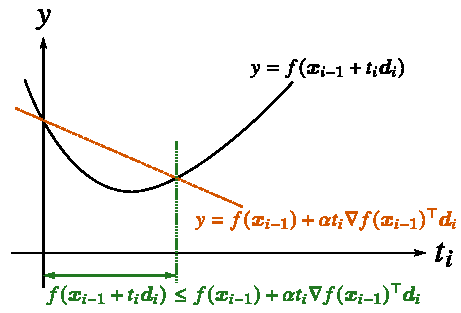
\includegraphics[width=0.7\linewidth]{optimization/Armijo-rule-image.pdf}
    \caption{Armijo の条件(式\eqref{optimization_unconstrained_descent-methods_Armijo-rule})のイメージ}
    \label{fig::optimization_unconstrained_descent-methods_Armijo-rule-image}
\end{figure}

Backtracking Line Search \cite[Section 9.2]{Boyd2004} は
Armijo の条件 \cite[Section 7.5]{Luenberger2003}
\begin{equation}
    f(\bm{x}_{i-1} + t_i \bm{d}_i) \le f(\bm{x}_{i-1}) + \alpha t_i \nabla f(\bm{x}_{i-1})^\top \bm{d}_i
    \label{eq:optimization_unconstrained_descent-methods_Armijo-rule}
\end{equation}
を利用する.
ここで,$\alpha$ は $\alpha \in (0,1)$ を満たす定数であり,
Armijo の条件は,
図\ref{fig:optimization_unconstrained_descent-methods_Armijo-rule-image}のように
十分小さい $t_i$ を選択するための条件となっている.
Backtracking Line Search では,
$\alpha \in (0, 1/2)$ とし,
Algorithm \ref{alg:optimization_unconstrained_descent-methods_BacktrackingLineSearch}
のように
$t_i$ を初期値 1 から $\beta \in (0, 1)$ 倍していき,
式 \eqref{eq:optimization_unconstrained_descent-methods_Armijo-rule} を満たすものを探索する.
一般に,パラメータ $\alpha$, $\beta$ は
$\alpha \in [0.01, 0.3]$, $\beta \in [0.1, 0.8]$ の範囲で設定される
\cite[Section 9.2]{Boyd2004}.

\subsection{最急降下法}

最急降下法では,更新方向を $\bm{d}_i = -\nabla f(\bm{x}_{i-1})$ とする.
確実に目的関数の減少する方向を示しており,
ここで示す他のアルゴリズムよりも更新方向の算出が簡単である.
目的関数が強凸関数である場合において,
最適解への収束が証明されている
\cite[Section 9.3.1]{Boyd2004}.

\subsection{Newton 法}

Newton 法では,
目的関数が狭義凸関数である(つまり,Hessian $\nabla^2 f(\bm{x}_{i-1})$ が正定値である)場合を対象とし,
更新方向を
$\bm{d}_i = -\nabla^2 f(\bm{x}_{i-1})^{-1} \nabla f(\bm{x}_{i-1})$
とする.
$\nabla^2 f(\bm{x}_{i-1})$ が正定値である場合,
$\nabla^2 f(\bm{x}_{i-1})^{-1}$ も正定値になる
\footnote{%
対称行列 $A$ が正定値である場合,$A$ の固有値は正の実数である.%
$A$ は固有値分解により $A=VDV^\top$ ($D$ は固有値による対角行列,$V$ は直交行列)と書くことができるため,%
$A^{-1} = VD^{-1}V^\top$ となる.%
よって,$A^{-1}$ の固有値も全て正の実数であり,%
$A^{-1}$ は正定値である.%
}
ため,
最適解でない $\bm{x}_{i-1}$ においては
$\nabla f(\bm{x}_{i-1})^\top \bm{d}_i = -\nabla f(\bm{x}_{i-1})^\top \nabla^2 f(\bm{x}_{i-1})^{-1} \nabla f(\bm{x}_{i-1}) < 0$
となり,目的関数が減少する方向になっていることを確認できる.
Newton 法の収束性については \cite[Section 9.5.3, 9.6.4]{Boyd2004} にて議論されている.

\subsection{準 Newton 法}

Newton 法では,
Hessian $\nabla^2 f(\bm{x}_{i-1})$ の逆行列が必要になるが,
$x^4$ のように 2 階微分が 0 になる点があったり,
Hessian の逆行列を安定的に計算できない点があったりする場合には使用できない.
そこで,Newton 法の更新方向
$\bm{d}_i = -\nabla^2 f(\bm{x}_{i-1})^{-1} \nabla f(\bm{x}_{i-1})$
における Hessian を
$\bm{d}_i = -H_{i-1} \nabla f(\bm{x}_{i-1})$
のように Hessian の代わりの行列で置き換える準 Newton 法と呼ばれるアルゴリズムがある.

準 Newton 法のうち,
Davidon-Fletcher-Powell (DFP) 公式では次のように $H_i$ を算出する
\cite[Section 9.3]{Luenberger2003}, \cite[Section 10.9]{Press2007}.
\begin{align}
    H_{i+1} &= H_i + \frac{\bm{p}_i \bm{p}_i^\top}{\bm{p}_i^\top \bm{q}_i}
        - \frac{H_i \bm{q}_i \bm{q}_i^\top H_i}{\bm{q}_i^\top H_i \bm{q}_i} \\
    \bm{p}_i &= \bm{x}_{i+1} - \bm{x}_i \\
    \bm{q}_i &= \nabla f(\bm{x}_{i+1}) - \nabla f(\bm{x}_i)
\end{align}
初期値 $H_0$ を対称な正定値の行列にしておけば,
全ての $H_i$ が帰納的に正定値になる
\cite[Section 9.3]{Luenberger2003}.
$H_i$ が正定値であれば,更新方向 $\bm{d}_i$ は目的関数の減少する方向になる.

また,同様の性質を持つ公式の 1 つとして,
Broyden-Fletcher-Goldfarb-Shanno (BFGS) 公式が存在する
\cite[Section 9.4]{Luenberger2003}.
\begin{align}
    H_i &= B_i^{-1} \\
    B_{i+1} &= B_i + \frac{\bm{q}_i \bm{q}_i^\top}{\bm{q}_i^\top \bm{p}_i}
        - \frac{B_i \bm{p}_i \bm{p}_i^\top B_i}{\bm{p}_i^\top B_i \bm{p}_i}
\end{align}
逆行列を計算することで次のようにも書くことができる
\cite[Section 10.9]{Press2007}.
\begin{align}
    H_{i+1} &= H_i + \frac{\bm{p}_i \bm{p}_i^\top}{\bm{p}_i^\top \bm{q}_i}
        - \frac{H_i \bm{q}_i \bm{q}_i^\top H_i}{\bm{q}_i^\top H_i \bm{q}_i}
        + \bm{q}_i^\top H_i \bm{q}_i \bm{v}_i \bm{v}_i^\top \\
    \bm{v}_i &= \frac{\bm{p}_i}{\bm{p}_i^\top \bm{q}_i}
        - \frac{H_i \bm{q}_i}{\bm{q}_i^\top H_i \bm{q}_i}
\end{align}

\subsection{共役勾配法}

共役勾配法では,
\begin{align}
    \bm{d}_1 &= -\nabla f(\bm{x}_{i-1}) \\
    \bm{d}_i &= -\nabla f(\bm{x}_{i-1}) + \gamma_i \bm{d}_{i-1} \\
    \gamma_i &= 
        \frac{(\nabla f(\bm{x}_{i-1}) - \nabla f(\bm{x}_{i-2}))^\top \nabla f(\bm{x}_{i-1})}
        {\|\nabla f(\bm{x}_{i-2})\|_2^2}
\end{align}
のように更新方向を算出する
\cite[Section 8.6]{Luenberger2003}.
$\gamma_i$ については複数の形式があるが,
ここで示している Polak-Ribiere 法は一般により良い結果が得られるという
\cite[Section 8.6]{Luenberger2003}, \cite[Section 10.8]{Press2007}.
Newton 法では計算量の多い逆行列の計算が必要だが,
共役勾配法では計算量が変数の次元のオーダーに収まるため,
各反復の計算時間を抑えられる.



% !TEX root = ../main.tex
%

\part{常微分方程式の数値解法}

\chapter{導入}

\index{じょうびぶんほうていしき@常微分方程式}
\index{ordinary differential equation|see{常微分方程式}}
この部では,常微分方程式 (ordinary differential equation, ODE) の数値解法をまとめる.

関数 $\bm{y}(t)$ の常微分方程式は一般に
\begin{equation}
    \bm{f}(t, \bm{y}, \dot{\bm{y}}, \ddot{\bm{y}}, \dddot{\bm{y}}, \ddddot{\bm{y}}, \ldots) = \bm{0}
\end{equation}
のように書ける.

% !TEX root = ../main.tex
%

\chapter{Runge-Kutta 法}

Runge-Kutta 法 (Runge-Kutta method) では次のような形式の初期値問題を数値的に解く
\cite{Mitsui1993}.
\begin{equation}
    \begin{cases}
        \dot{\bm{y}} = \bm{f}(t, \bm{y}) \\
        \bm{y}(0) = \bm{y}_0
    \end{cases}
\end{equation}

Runge-Kutta 法は,時刻 $t$ における変数 $\bm{y}(t)$ の値から,
次のような形式で時刻 $t + h$ における変数 $\bm{y}(t + h)$ の計算を行う.
\begin{align}
    \bm{k}_i      & = \bm{f}\left(t + c_i h, \bm{y}(t) + h \sum_{j = 1}^s a_{ij} \bm{k}_j \right)
                  & \text{for $i = 1, 2, \ldots, s$}
    \label{eq:ode_runge-kutta_k-law}                                                              \\
    \bm{y}(t + h) & = \bm{y}(t) + \sum_{i=1}^s b_i \bm{k}_i
    \label{eq:ode_runge-kutta_y-law}
\end{align}

ここで,時間の更新幅 $h$ はステップ幅と呼ばれる.
Runge-Kutta 法には,
整数 $s$ (段数と呼ばれる)と係数 $a_{ij}$, $b_i$, $c_i$ の異なる様々な公式が存在する.
係数 $a_{ij}$, $b_i$, $c_i$ は
表 \ref{table:ode_runge-kutta_butcher-array-general} のような
Butcher 配列と呼ばれる形式で記載される.

\begin{table}[bp]
    \caption{Butcher 配列における係数の並べ方}
    \label{table:ode_runge-kutta_butcher-array-general}
    \centering
    \begin{tabular}{c|ccccc}
        $c_1$    & $a_{11}$ & $a_{12}$ & $a_{13}$ & $\cdots$ & $a_{1s}$ \\
        $c_2$    & $a_{21}$ & $a_{22}$ & $a_{23}$ & $\cdots$ & $a_{2s}$ \\
        $c_3$    & $a_{31}$ & $a_{32}$ & $a_{33}$ & $\cdots$ & $a_{3s}$ \\
        $\vdots$ & $\vdots$ & $\vdots$ & $\vdots$ & $\ddots$ & $\vdots$ \\
        $c_s$    & $a_{s1}$ & $a_{s2}$ & $a_{s3}$ & $\cdots$ & $a_{ss}$ \\
        \hline
                 & $b_1$    & $b_2$    & $b_3$    & $\cdots$ & $b_s$
    \end{tabular}
\end{table}

Runge-Kutta 法の公式は次のように分類される.

\begin{description}
    \item[陽的 Runge-Kutta 法] $j \ge i$ について $a_{ij} = 0$ となっている場合,
          $\bm{k}i$ は $\bm{k}_1, \bm{k}_2, \ldots, \bm{k}_s$
          の順に式 \eqref{eq:ode_runge-kutta_k-law} の右辺を評価することで計算できる.
          このような場合は陽的 Runge-Kutta 法と呼ばれる.
    \item[半陰的 Runge-Kutta 法] $j > i$ について $a_{ij} = 0$ となっている場合,
          $\bm{k}i$ は $\bm{k}_1, \bm{k}_2, \ldots, \bm{k}_s$
          の順に式 \eqref{eq:ode_runge-kutta_k-law} を $\bm{k}_i$ について解くことで計算できる.
          このような場合は半陰的 Runge-Kutta 法と呼ばれる.
    \item[陰的 Runge-Kutta 法] $j > i$ でも $a_{ij} \neq 0$ となる係数が存在する場合,
          $\bm{k}i$ は $i = 1, 2, \ldots, s$ について連立した
          式 \eqref{eq:ode_runge-kutta_k-law} を $\bm{k}_i$ について解くことで計算する.
          このような場合は陰的 Runge-Kutta 法と呼ばれる.
\end{description}

陽的 Runge-Kutta 法の方が計算は単純だが,
陰的 Runge-Kutta 法は

\begin{itemize}
    \item 硬い系と呼ばれる比較的不安定な微分方程式で解が安定しやすい.
    \item 陽的 Runge-Kutta 法よりも少ない段数でより高い次数を出せる.
          (後述する公式の実例を見ると分かる.)
\end{itemize}

といった利点を持つ.
そのため,解が安定するようにステップ幅を調整した場合,
陰的 Runge-Kutta 法の方がステップ幅を大きくとることができ,
目的の時刻 $t$ までの解を得るために必要な計算時間は少なくなる場合がある.

また,Runge-Kutta 法の公式の精度を示す数値として次数が存在する.
変数の近似値 $\bm{y}(t + h)$ の精度が $h^p$ オーダーの場合,
その公式は $p$ 次といい,$p$ は次数と呼ばれる.

\section{埋め込み型公式}

Runge-Kutta 法の公式の中には,複数の $b_i$ の組を持つものがある
(表 \ref{table:ode_runge-kutta_butcher-array-rkf45} の例を参照).
そのような公式では,次のような 2 つの近似値を得ることができる.
\begin{align}
    \bm{y}(t + h)   & = \bm{y}(t) + \sum_{i=1}^s b_i \bm{k}_i     \\
    \bm{y}^*(t + h) & = \bm{y}^*(t) + \sum_{i=1}^s b_i^* \bm{k}_i
\end{align}
これらの差により誤差の近似値を求めることができる.
\begin{align}
    \bm{y}(t + h) - \bm{y}^*(t + h) & = \sum_{i=1}^s (b_i - b_i^*) \bm{k}_i
\end{align}

これを用いると,現在のステップ幅から次のステップ幅 $\hat{h}$ の適正値を推定できる.
まず,$b_i$ と $b_i^*$ のうち次数が低い方の次数を $p$ とすると,
\begin{align}
    \left| \bm{y}(t + h) - \bm{y}^*(t + h) \right| \approx |Ah^p|
\end{align}
のように書ける.
そこで,誤差の許容量を $\epsilon_{tol}$ としたとき,次の方程式が成り立つようにする.
\begin{equation}
    \frac{\hat{h}^p}{h^p} = \frac{\epsilon_{tol}}{\left| \bm{y}(t + h) - \bm{y}^*(t + h) \right|}
\end{equation}
これを $\hat{h}$ について解くと,次のようになる.
\begin{equation}
    \hat{h} = h \left(\frac{\epsilon_{tol}}{\left| \bm{y}(t + h) - \bm{y}^*(t + h) \right|}\right)^{\frac{1}{p}}
\end{equation}

\section{古典的 Runge-Kutta 法}

\begin{table}[bp]
    \caption{古典的 Runge-Kutta 法 (RK4 公式)の Butcher 配列}
    \label{table:ode_runge-kutta_butcher-array-rk4}
    \centering
    \begin{tabular}{c|cccc}
        $0$           &               &               &               &               \\
        $\frac{1}{2}$ & $\frac{1}{2}$ &               &               &               \\
        $\frac{1}{2}$ & $0$           & $\frac{1}{2}$ &               &               \\
        $1$           & $0$           & $0$           & $1$           &               \\
        \hline
                      & $\frac{1}{6}$ & $\frac{1}{3}$ & $\frac{1}{3}$ & $\frac{1}{6}$
    \end{tabular}
\end{table}

古典的 Runge-Kutta 法と呼ばれる公式では,
表 \ref{table:ode_runge-kutta_butcher-array-rk4} のような係数を用いる
\cite[3.3 節]{Mitsui1993}.
単純な係数で次数 4 を達成できる.

\section{RKF45 公式}

\begin{table}[bp]
    \caption{RKF45 公式の Butcher 配列}
    \label{table:ode_runge-kutta_butcher-array-rkf45}
    \centering
    \begin{tabular}{c|ccccccc}
        $0$             &                     &                      &                      &                       &                  &                &          \\
        $\frac{1}{4}$   & $\frac{1}{4}$       &                      &                      &                       &                  &                &          \\
        $\frac{3}{8}$   & $\frac{3}{32}$      & $\frac{9}{32}$       &                      &                       &                  &                &          \\
        $\frac{12}{13}$ & $\frac{1932}{2197}$ & $-\frac{7200}{2197}$ & $\frac{7296}{2197}$  &                       &                  &                &          \\
        $1$             & $\frac{439}{216}$   & $-8$                 & $\frac{3680}{513}$   & $-\frac{845}{4104}$   &                  &                &          \\
        $\frac{1}{2}$   & $-\frac{8}{27}$     & $2$                  & $-\frac{3544}{2565}$ & $\frac{1859}{4104}$   & $-\frac{11}{40}$ &                &          \\
        \hline
                        & $\frac{16}{135}$    & $0$                  & $\frac{6656}{12825}$ & $\frac{28561}{56430}$ & $-\frac{9}{50}$  & $\frac{2}{55}$ & (5 次) \\
                        & $\frac{25}{216}$    & $0$                  & $\frac{1408}{2565}$  & $\frac{2197}{4104}$   & $-\frac{1}{5}$   & $0$            & (4 次)
    \end{tabular}
\end{table}

RKF45 公式(RKF は Runge-Kutta-Fehlberg のこと)では,
表 \ref{table:ode_runge-kutta_butcher-array-rkf45} のような係数を用いる
\cite[4.1 節 (a)]{Mitsui1993}, \cite[Section 9.5]{Mathews2004}.
この埋め込み型公式では,$\bm{k}_i$ から $\bm{y}(t + h)$ を算出する係数に
5 次の精度を持つ組と 4 次の精度を持つ組が存在する
\footnote{挙げた 2 件の文献のうち,%
    文献 \cite{Mitsui1993} では係数が一カ所誤っていたため注意が必要.}.

\section{田中公式}

\begin{table}[bp]
    \caption{田中 Formula1 公式の Butcher 配列}
    \label{table:ode_runge-kutta_butcher-array-tanaka-formula1}
    \centering
    \begin{tabular}{c|ccc}
        $\frac{13}{20}$ & $\frac{13}{20}$    &                  &          \\
        $-\frac{1}{18}$ & $-\frac{127}{180}$ & $\frac{13}{20}$  &          \\
        \hline
                        & $\frac{100}{127}$  & $\frac{27}{127}$ & (3 次) \\
                        & $1$                &                  & (1 次)
    \end{tabular}
\end{table}

\begin{table}[bp]
    \caption{田中 Formula2 公式の Butcher 配列}
    \label{table:ode_runge-kutta_butcher-array-tanaka-formula2}
    \centering
    \begin{tabular}{c|cccc}
        $\frac{133}{100}$ & $\frac{133}{100}$     &                       &                      &          \\
        $\frac{1}{2}$     & $-\frac{5400}{18167}$ & $\frac{28967}{36334}$ &                      &          \\
        $-\frac{33}{100}$ & $\frac{133}{50}$      & $-\frac{108}{25}$     & $\frac{133}{100}$    &          \\
        \hline
                          & $\frac{1250}{20667}$  & $\frac{18167}{20667}$ & $\frac{1250}{20667}$ & (4 次) \\
                          & $0$                   & $1$                   &                      & (2 次)
    \end{tabular}
\end{table}

文献 \cite{Togawa2007} では,田中正次氏が考案した半陰的・陰的公式がいくつか示されている.
そのうち埋め込み型の半陰的公式を表
\ref{table:ode_runge-kutta_butcher-array-tanaka-formula1},
\ref{table:ode_runge-kutta_butcher-array-tanaka-formula2}
に示す
\footnote{文献 \cite{Togawa2007} には完全に陰的な 4 段 7 次の公式もあるが,%
    係数がかなり複雑なため省略した.}.

段数の多い陽的公式と同程度の精度を少ない段数で出すことができていることを確認できる.
また,埋め込み型の 2 つの係数のうち次数の低い方の係数が単純になっている
\footnote{利用する際には高い次数の係数との差を見るように実装するため,%
    次数の低い方の係数だけ単純でも計算コストへの影響はない.}.

\section{Butcher-Kuntzmann 公式}

\begin{table}[bp]
    \caption{2 段 Butcher-Kuntzmann 公式の Butcher 配列}
    \label{table:ode_runge-kutta_butcher-array-2stage-butcher-kuntzmann}
    \centering
    \begin{tabular}{c|cc}
        $\frac{1}{2} + \frac{\sqrt{3}}{6}$ & $\frac{1}{4}$                      & $\frac{1}{4} + \frac{\sqrt{3}}{6}$ \\
        $\frac{1}{2} - \frac{\sqrt{3}}{6}$ & $\frac{1}{4} - \frac{\sqrt{3}}{6}$ & $\frac{1}{4}$                      \\
        \hline
                                           & $\frac{1}{2}$                      & $\frac{1}{2}$
    \end{tabular}
\end{table}

文献 \cite[5.2 節 (b)]{Mitsui1993} によると,
陰的 Runge-Kutta 法では,$s$ 段公式で $2s$ 次を超えることができないと証明されており,
その限界の $2s$ 次の公式が存在することも証明されている.
特に Legendre 関数の零点を用いて係数を決める種類の公式は,
$s$ 段 Butcher-Kuntzmann 公式と呼ばれる.
2 段 Butcher-Kuntzmann 公式を表
\ref{table:ode_runge-kutta_butcher-array-2stage-butcher-kuntzmann}
に示す(前述の通り 4 次の精度を持つ).

\section{Euler 法}

\begin{table}[bp]
    \caption{Euler 法の Butcher 配列}
    \label{table:ode_runge-kutta_butcher-array-explicit-euler}
    \centering
    \begin{tabular}{c|c}
        $1$ &     \\
        \hline
            & $1$
    \end{tabular}
\end{table}

常微分方程式の解法としては最も基本的な Euler 法
\begin{equation}
    \bm{y}(t + h) \approx \bm{y}(t) + h \bm{f}(t, \bm{y}(t))
\end{equation}
は形式的に Runge-Kutta 法とみなすことができる.
Butcher 配列は表 \ref{table:ode_runge-kutta_butcher-array-explicit-euler} に示す通りである.

% !TEX root = ../main.tex
%

\chapter{平均ベクトル場法}

エネルギー保存則を満たす系の運動方程式を解くことを目的とした手法の 1 つとして,
平均ベクトル場法(Average vector field method, AVF method) \cite{Quispel2008} がある.

座標 $\bm{q}$ に対して,
運動エネルギーが $T = \bm{p}^\top \dot{\bm{q}} / 2$ で表現されるようにモーメント $\bm{p}$ を定める.
さらに位置エネルギー $V$ を座標 $\bm{q}$ で表現することで,
全エネルギーの和を表現した関数 $H(\bm{q}, \bm{p}) = T + V$ を
ハミルトニアン(Hamiltonian)と呼ぶ
\cite[Section 3.2]{Morse1953}.
このとき,運動方程式は次の式で表現される.
\begin{align}
    \dot{\bm{q}} & = \frac{\partial H}{\partial \bm{p}}  \\
    \dot{\bm{p}} & = -\frac{\partial H}{\partial \bm{q}}
\end{align}
この式は変数 $\bm{y} = (\bm{q}^\top, \bm{p}^\top)^\top$ を用いて次のように書くこともできる.
\begin{equation}
    \dot{\bm{y}} = \bm{f}(\bm{y}) \equiv S \nabla H(\bm{y})
\end{equation}
文献 \cite{Quispel2008} はこの形式の微分方程式を前提として
次のような数値解法を提案している.
\begin{equation}
    \frac{\bm{y}_{n+1} - \bm{y}_n}{h}
    = \int_{0}^{1} \bm{f}((1 - \xi) \bm{y}_n + \xi \bm{y}_{n+1}) d \xi
    \label{eq:ode_average-vector-field_update-2-order}
\end{equation}

この手法がエネルギーを保存することを示す.
まず,$\bm{f}(\bm{y}) \equiv S \nabla H(\bm{y})$ より
\begin{equation}
    \frac{\bm{y}_{n+1} - \bm{y}_n}{h}
    = S \int_{0}^{1} \nabla H((1 - \xi) \bm{y}_n + \xi \bm{y}_{n+1}) d \xi
    \label{eq:ode_average-vector-field_update-with-hamiltonian}
\end{equation}
である.ここで,$S$ は
\begin{equation}
    S =
    \begin{pmatrix}
        O  & I \\
        -I & O
    \end{pmatrix}
\end{equation}
であるため
\footnote{このような行列は歪対称行列と呼ばれる.}
,任意のベクトル $\bm{y} = (\bm{q}^\top, \bm{p}^\top)^\top$ において,
\begin{equation}
    \bm{y}^\top S \bm{y} =
    \begin{pmatrix}
        \bm{q}^\top & \bm{p}^\top
    \end{pmatrix}
    \begin{pmatrix}
        O  & I \\
        -I & O
    \end{pmatrix}
    \begin{pmatrix}
        \bm{q} \\ \bm{p}
    \end{pmatrix}
    =
    \begin{pmatrix}
        \bm{q}^\top & \bm{p}^\top
    \end{pmatrix}
    \begin{pmatrix}
        \bm{p} \\ -\bm{q}
    \end{pmatrix}
    = \bm{0}
\end{equation}
となる.よって,
式 \eqref{eq:ode_average-vector-field_update-with-hamiltonian}
の両辺と
$\int_{0}^{1} \nabla H((1 - \xi) \bm{y}_n + \xi \bm{y}_{n+1}) d \xi$ の内積をとると
\begin{equation}
    \frac{\bm{y}_{n+1} - \bm{y}_n}{h}
    \int_{0}^{1} \nabla H((1 - \xi) \bm{y}_n + \xi \bm{y}_{n+1}) d \xi
    = 0
\end{equation}
となる.さらに左辺は
\begin{align}
      & \frac{\bm{y}_{n+1} - \bm{y}_n}{h}
    \int_{0}^{1} \nabla H((1 - \xi) \bm{y}_n + \xi \bm{y}_{n+1}) d \xi         \\
    = & \frac{1}{h}
    \int_{0}^{1} \frac{d}{d\xi} H((1 - \xi) \bm{y}_n + \xi \bm{y}_{n+1}) d \xi \\
    = & \frac{H(\bm{y}_{n+1}) - H()\bm{y}_{n})}{h}
\end{align}
と変形できるから,次のようにエネルギーの保存が示される.
\begin{equation}
    H(\bm{y}_{n+1}) - H(\bm{y}_{n}) = 0
\end{equation}

式 \eqref{eq:ode_average-vector-field_update-2-order} は 2 次の精度だが,
3 次と 4 次の公式も文献 \cite{Quispel2008} で示されている.
それらは次の式で与えられる.
\begin{equation}
    \frac{\bm{y}_{n+1} - \bm{y}_n}{h}
    = \left(I + \alpha h^2
    \left(\left. \frac{\partial \bm{f}}{\partial \bm{y}} \right|_{\bm{y} = \hat{\bm{y}}}\right)^2
    \right)
    \int_{0}^{1} \bm{f}((1 - \xi) \bm{y}_n + \xi \bm{y}_{n+1}) d \xi
\end{equation}
パラメータと次数は次のようになる.
\begin{itemize}
    \item $\alpha = 0$ とすると 2 次精度の更新式
          \eqref{eq:ode_average-vector-field_update-2-order}
          が得られる.
    \item $\alpha = -1/12$, $\hat{\bm{y}} = \bm{y}_n$ とすると
          3 次精度の更新式が得られる.
    \item $\alpha = -1/12$, $\hat{\bm{y}} = (\bm{y}_n + \bm{y}_{n+1})/2$ とすると
          4 次精度の更新式が得られる.
\end{itemize}

この手法の更新式は次数に依らず陰的で,
次数が上がるごとに計算が複雑になっていく.
ここで,次数 2 のときの方程式
\begin{equation}
    F(\bm{y}_{n+1}) \equiv
    \frac{\bm{y}_{n+1} - \bm{y}_n}{h} -
    \int_{0}^{1} \bm{f}((1 - \xi) \bm{y}_n + \xi \bm{y}_{n+1}) d \xi
    = 0
\end{equation}
を考える.
これを Newton-Raphson 法(\ref{chap:root-finding_newton-raphson} 章)で解くには,
Jacobian が必要となる.
Jacobian は次のようになる.
\begin{equation}
    \frac{\partial F}{\partial \bm{y}_{n+1}} =
    \frac{1}{h} I -
    \int_{0}^{1} \xi \left. \frac{\partial \bm{f}}{\partial \bm{y}} \right|_{\bm{y} = (1 - \xi) \bm{y}_n + \xi \bm{y}_{n+1}} d \xi
\end{equation}
さらに,Jacobian の変化が十分小さいとすると,
\begin{align}
            & \frac{\partial F}{\partial \bm{y}_{n+1}}                                                \\
    \approx & \frac{1}{h} I -
    \int_{0}^{1} \xi \left. \frac{\partial \bm{f}}{\partial \bm{y}} \right|_{\bm{y} = \bm{y}_n} d \xi \\
    =       & \frac{1}{h} I - \frac{1}{2}
    \left. \frac{\partial \bm{f}}{\partial \bm{y}} \right|_{\bm{y} = \bm{y}_n}
    \label{eq:ode_average-vector-field_approx-jacobian}
\end{align}
のように近似できる.
3 次と 4 次の更新式でも,Newton-Raphson 法の Jacobian においては $h^2$ の項を無視して
式 \eqref{eq:ode_average-vector-field_approx-jacobian} で
近似することができる.


% !TEX root = ../main.tex
%

\part{高精度演算}

% !TEX root = ../main.tex
%

\chapter{倍精度浮動小数点数による多倍長浮動小数点数}

倍精度浮動小数点数を用いて四倍精度,八倍精度といったより高い精度の演算を行う手法が考えられている
\cite{Hirayama2014,Hida2001}.
それぞれ 2 つ,4 つの倍精度浮動小数点数の和で小数を表現し,
仮数の桁が被らないように演算することで高い精度を実現する.

\section{記号}

本章で使用する記号を以下に示す.

\begin{explainlist}
    $\oplus$ & 倍精度浮動小数点数の加算 \\
    $\ominus$ & 倍精度浮動小数点数の減算 \\
    $\otimes$ & 倍精度浮動小数点数の乗算 \\
    $\oslash$ & 倍精度浮動小数点数の除算 \\
\end{explainlist}

\section{基本演算}

倍精度浮動小数点数による四倍精度,八倍精度演算の既存文献\cite{Hida2001}で使用される
基本的な演算を以下にまとめる.

まず,$|a| \ge |b|$ となる倍精度浮動小数点数 $a$, $b$ について
$s = a \oplus b$, $a + b = s + e$ が成り立つ倍精度浮動小数点数 $s$, $e$ を
算出するアルゴリズムを Algorithm \ref{more-precision_multi-double_algo_QuickTwoSum} に示す.
なお,$a$, $b$ の大小が不明な場合は
Algorithm \ref{more-precision_multi-double_algo_TwoSum} を使用する.

\begin{algorithm}[tp]
    \caption{大小の明確な倍精度浮動小数点数の加算と誤差計算\cite[Algorithm 3]{Hida2001}}
    \label{more-precision_multi-double_algo_QuickTwoSum}
    \begin{algorithmic}[1]
        \Procedure{QuickTwoSum}{$a, b$}
        \State $s \gets a \oplus b$
        \State $e \gets b \ominus (s \ominus a)$
        \State \Return $(s, e)$
        \EndProcedure
    \end{algorithmic}
\end{algorithm}

\begin{algorithm}[tp]
    \caption{大小の不明な倍精度浮動小数点数の加算と誤差計算\cite[Algorithm 4]{Hida2001}}
    \label{more-precision_multi-double_algo_TwoSum}
    \begin{algorithmic}[1]
        \Procedure{TwoSum}{$a, b$}
        \State $s \gets a \oplus b$
        \State $v \gets s \ominus a$
        \State $e \gets (a \ominus (s \ominus v)) \oplus (b \ominus v)$
        \State \Return $(s, e)$
        \EndProcedure
    \end{algorithmic}
\end{algorithm}

また,乗算についても
$s = a \otimes b$, $a \times b = s + e$ となる
倍精度浮動小数点数 $s$, $e$ を算出する
Algorithm \ref{more-precision_multi-double_algo_TwoProd} が存在する.
ただし,fused multiply-add (FMA) 命令が存在する CPU では,
Algorithm \ref{more-precision_multi-double_algo_TwoProdFMA} により高速化が期待できる.

\begin{algorithm}[tp]
    \caption{倍精度浮動小数点数の乗算と誤差計算\cite[Algorithm 5, 6]{Hida2001}}
    \label{more-precision_multi-double_algo_TwoProd}
    \begin{algorithmic}[1]
        \Procedure{TwoProd}{$a, b$}
        \State $p \gets a \otimes b$
        \State $(a_h, a_l) \gets \text{Split}(a)$
        \State $(b_h, b_l) \gets \text{Split}(b)$
        \State $e \gets ((a_h \otimes b_h \ominus p) \oplus a_h \otimes b_l \oplus a_l \otimes b_h) \oplus a_l \otimes b_l$
        \State \Return $(p, e)$
        \EndProcedure
    \end{algorithmic}
    \begin{algorithmic}[1]
        \Procedure{Split}{$a$}
        \State $t \gets (2^{27} + 1) \otimes a$
        \State $a_h \gets t \ominus (t \ominus a)$
        \State $a_l \gets a \ominus a_h$
        \State \Return $(a_h, a_l)$
        \EndProcedure
    \end{algorithmic}
\end{algorithm}

\begin{algorithm}[tp]
    \caption{倍精度浮動小数点数の乗算と誤差計算(FMA 命令を使用する場合)\cite[Algorithm 7]{Hida2001}}
    \label{more-precision_multi-double_algo_TwoProdFMA}
    \begin{algorithmic}[1]
        \Procedure{TwoProdFMA}{$a, b$}
        \State $s \gets a \otimes b$
        \State $e \gets \text{FMA}(a, b, -p)$
        \Comment{$\text{FMA}(a, b, c)$ は $a \times b + c$ を $a \times b$ を途中で丸めずに計算する.}
        \State \Return $(s, e)$
        \EndProcedure
    \end{algorithmic}
\end{algorithm}

\clearpage

\section{倍精度浮動小数点数による四倍精度演算}

四倍精度浮動小数点数を $a = a_h + a_l$, $|a_l| \le (1/2) \ulp(|a_h|)$ となる
倍精度浮動小数点数 $a_h$, $a_l$ で表現する.

\subsection{四則演算}

このとき,加算は
Algorithm \ref{more-precision_multi-double_algo_QuadAddPrecisely},
\ref{more-precision_multi-double_algo_QuadAddSimple}
のようなアルゴリズムで行うことができる.
Algorithm \ref{more-precision_multi-double_algo_QuadAddSimple} の方が
簡潔な演算手法だが,
倍精度浮動小数点数の 2 倍の 104 ビットの精度で演算できることが
示されている\cite{Naoya2012}.
減算も加算と同様にして行うことができる.

\begin{algorithm}[tp]
    \caption{四倍精度の加算(正確な演算)\cite{Hisashi2006}}
    \label{more-precision_multi-double_algo_QuadAddPrecisely}
    \begin{algorithmic}[1]
        \Procedure{QuadAddPrecisely}{$(a_h, a_l), (b_h, b_l)$}
        \State $(x_h, x_l) \gets \text{TwoSum}(a_h, b_h)$
        \State $(y_h, y_l) \gets \text{TwoSum}(a_l, b_l)$
        \State $x_l \gets x_l \oplus y_h$
        \State $(x_h, x_l) \gets \text{QuickTwoSum}(x_h, x_l)$
        \State $x_l \gets x_l \oplus y_l$
        \State $(x_h, x_l) \gets \text{QuickTwoSum}(x_h, x_l)$
        \State \Return $(x_h, x_l)$
        \EndProcedure
    \end{algorithmic}
\end{algorithm}

\begin{algorithm}[tp]
    \caption{四倍精度の加算(簡潔な演算)\cite{Naoya2012,Hirayama2014}}
    \label{more-precision_multi-double_algo_QuadAddSimple}
    \begin{algorithmic}[1]
        \Procedure{QuadAddSimple}{$(a_h, a_l), (b_h, b_l)$}
        \State $(x_h, x_l) \gets \text{TwoSum}(a_h, b_h)$
        \State $x_l \gets x_l \oplus a_l \oplus b_l$
        \State $(x_h, x_l) \gets \text{QuickTwoSum}(x_h, x_l)$
        \State \Return $(x_h, x_l)$
        \EndProcedure
    \end{algorithmic}
\end{algorithm}

また,乗算は
Algorithm \ref{more-precision_multi-double_algo_QuadMultiply} のようにすることで
102 ビットの精度で算出できることが示されている\cite{Naoya2012}.

\begin{algorithm}[tp]
    \caption{四倍精度の乗算\cite{Hisashi2006,Naoya2012}}
    \label{more-precision_multi-double_algo_QuadMultiply}
    \begin{algorithmic}[1]
        \Procedure{QuadMultiply}{$(a_h, a_l), (b_h, b_l)$}
        \State $(x_h, x_l) \gets \text{TwoProd}(a_h, b_h)$
        \State $x_l \gets x_l \oplus a_h \otimes b_l \oplus a_l \otimes b_h$
        \State $(x_h, x_l) \gets \text{QuickTwoSum}(x_h, x_l)$
        \State \Return $(x_h, x_l)$
        \EndProcedure
    \end{algorithmic}
\end{algorithm}

残りの四則演算である除算は
Algorithm \ref{more-precision_multi-double_algo_QuadDivide} のようにすることで
算出できる\cite{Naoya2012s}.

\begin{algorithm}[tp]
    \caption{四倍精度の除算\cite{Naoya2012s}}
    \label{more-precision_multi-double_algo_QuadDivide}
    \begin{algorithmic}[1]
        \Procedure{QuadDivide}{$(a_h, a_l), (b_h, b_l)$}
        \State $c \gets 1 \oslash b_h$
        \State $d \gets b_l \otimes c$
        \State $x_h \gets a_h \otimes c$
        \State $(r_1, r_2) \gets \text{TwoProd}(x_h, b_h)$
        \State $x_l \gets ((a_h \ominus r_1) \ominus r_2) \otimes c$
        \State $x_l \gets x_l \oplus x_h \otimes ((a_l \oslash a_h) \ominus d)$
        \State $(x_h, x_l) \gets \text{QuickTwoSum}(x_h, x_l)$
        \State \Return $(x_h, x_l)$
        \EndProcedure
    \end{algorithmic}
\end{algorithm}



%\section{テスト}
%
%テスト
%
%\begin{equation}
%    e^{ix} = \cos{x} + i \sin{x}
%\end{equation}
%
%\begin{lstlisting}[caption=テスト, language={C++}]
%int main() {
%    return 0; // 日本語コメント
%}
%\end{lstlisting}
%
%\begin{algorithm}
%    \caption{テスト}
%    \begin{algorithmic}
%        \Procedure{Test}{$x, y$}\Comment{テスト}
%        \State $x = y$
%        \EndProcedure
%    \end{algorithmic}
%\end{algorithm}
%
%\cite{Hirayama2014}

\bibliographystyle{junsrt}
\bibliography{articles.bib}

\end{document}
